\section{Removing Edges}
\label{sect:removing-edges}

\textbf{Remove edge on outer face:} Similarly, we can remove an edge $\{u, v\}$ on the outer face only if it doesn't create holes in the graph. This is the case iff $u$ and $v$ share a neighbor. The graph must also remain 2-connected.

\begin{figure}[H]
	\centering
	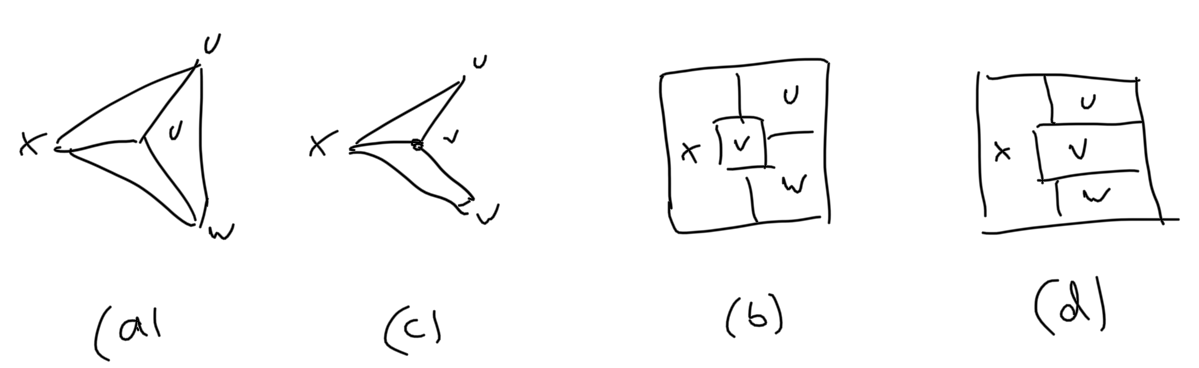
\includegraphics[height=30mm]{Resources/RemoveOuterEdge.png}
	\caption{A cluster graph and a polygonal dual thereof, before (a, b) and after (c, d) removing the edge $\{u,w\}$.}
	\label{fig:remove-outer-edge-example}
\end{figure}

%\begin{figure}[H]
%	\centering
%	\subfigure[]{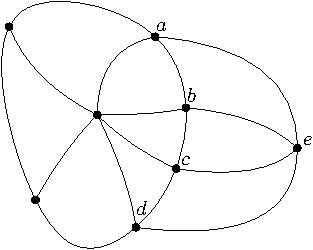
\includegraphics[height=30mm]{Resources/IncrementalFilteringAndEmbedding-RemoveOuterEdge-Initial.pdf}}
%	\quad
%	\subfigure[]{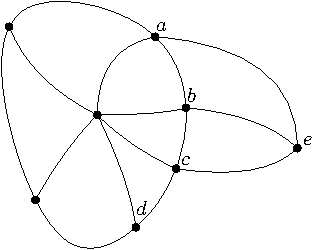
\includegraphics[height=30mm]{Resources/IncrementalFilteringAndEmbedding-RemoveOuterEdge-Valid.pdf}}
%	\quad
%	\subfigure[]{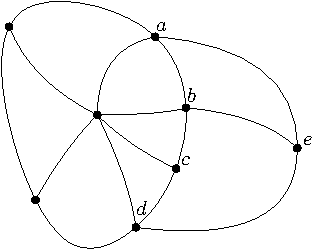
\includegraphics[height=30mm]{Resources/IncrementalFilteringAndEmbedding-RemoveOuterEdge-Invalid.pdf}}
%	\caption{Removing an edge on the outer face of an embedded filtered graph (a) correctly (b, edge $\{e,d\}$) and incorrectly, creating a 4-hole $bcde$ (edge $\{e,c\}$, c).}
%	\label{fig:transformation}
%\end{figure}
